\subsection{Résultats expérimentaux}
\label{result}
Nous analysons ici les premiers résultats de nos deux méthodes de résolution. Pour la résolution approchée, nous affichons ci-dessous les solutions trouvées à différentes étapes pour l'instance \texttt{A-n32-k5}:

\begin{center}
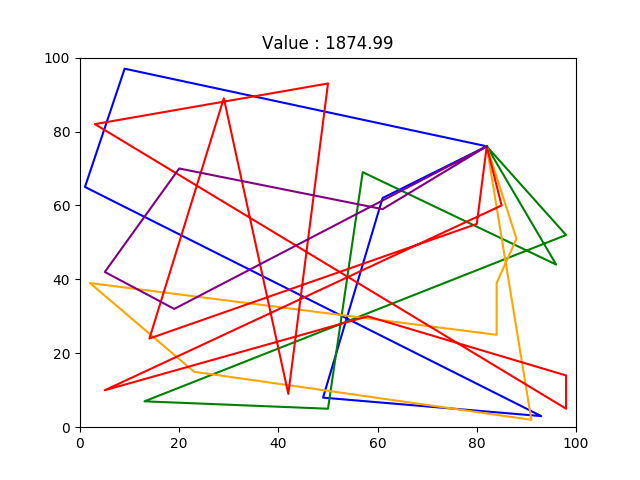
\includegraphics[width=0.32\linewidth]{pictures/image5.png}
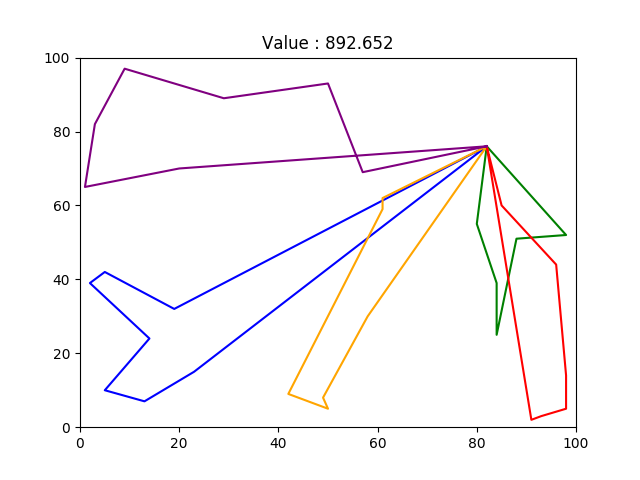
\includegraphics[width=0.32\linewidth]{pictures/image2.png}
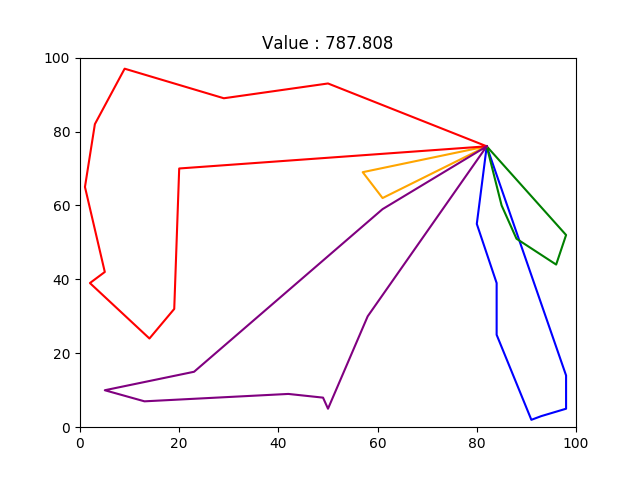
\includegraphics[width=0.32\linewidth]{pictures/image3.png}
\captionof{figure}{Tournées obtenues par : a) Construction b) Recuit simulé c) PLNE}
\end{center}

Dans la figure ci-dessus, nous pouvons voir en a) la solution obtenue après l'étape de construction. Cette solution est très éloignée et a une valeur de 1874. En b), nous avons la solution obtenue après l'algorithme du recuit simulé. Cette solution est bien plus approchée avec une valeur de 892. En c), nous avons la solution optimale avec une valeur de 787. De ces figures, nous pouvons voir que le recuit simulé améliore notre solution de départ et retourne une solution assez proche de la solution optimale. On peut notamment reconnaître des suites de clients dans certaines tournées.\\

Dans la figure ci-dessous, nous comparons les résultats obtenus par l'heuristique de construction, le recuit simulé et la résolution exacte \href{http://vrp.atd-lab.inf.puc-rio.br/index.php/en/}{des instances de type P}. Nous limitons le solveur à 300 secondes pour chaque instance.

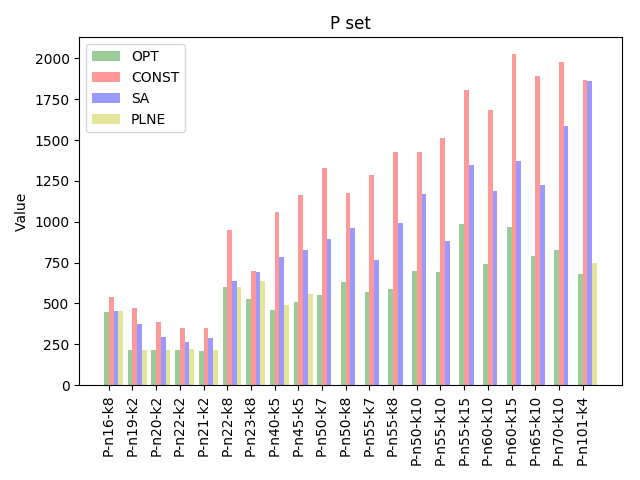
\includegraphics[width=0.8\textwidth]{pictures/image1.png}

Du fait de limiter le solveur à 300 secondes, nous remarquons que nous n'obtenons pas de résultat sur les grandes instances. Cela s'explique du fait que le nombre de contraintes de coupes augmente exponentiellement avec la taille de l'instance. Nous constatons que le recuit simulé renvoie des résultats beaucoup plus proche de l'optimum que l'heuristique de construction. Dans les cas plus difficiles, l'heuristique de recuit simulé nous donne des solutions réalisables avec un temps rapide. Pour les grandes instances, la résolution exacte prend plus de temps, mais donne de meilleurs résultats.